\documentclass[Ex4_Zusammenfassung.tex]{subfiles}

\begin{document}


\section{LS-Kopplung, jj-Kopplung}
\textbf{Von Heinstein und Anton}
\subsubsection*{LS-Kopplung}
\begin{itemize}
	\item Wasserstoff: Potential $\rightarrow$ Störungen $\rightarrow$ Spin-Bahn-Kopplung
	\item Spin-Bahn-Kopplung: nicht $\ell$ und $s$ sondern $j$ relevant
	\item Viele Elektronen: $J$ relevant
\end{itemize}

\begin{figure}[h]
	\centering
	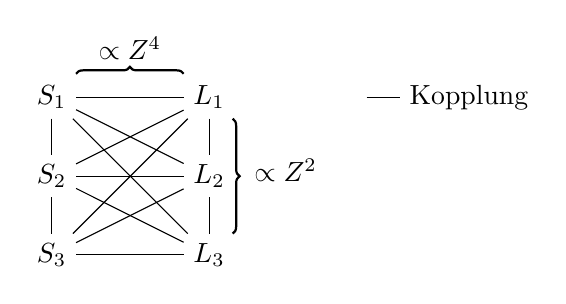
\begin{tikzpicture}
		\node at (0,0) (nodeS1) {$S_1$};
		\node at (0,-1) (nodeS2) {$S_2$};
		\node at (0,-2) (nodeS3) {$S_3$};
		\node at (2, 0) (nodeL1) {$L_1$};
		\node at (2, -1) (nodeL2) {$L_2$};
		\node at (2, -2) (nodeL3) {$L_3$};
		\node at (5.3, 0) (nodeK) {Kopplung};
		
		\draw (nodeS1) -- (nodeS2);
		\draw (nodeS2) -- (nodeS3);
		\draw (nodeS1) -- (nodeL1);
		\draw (nodeS1) -- (nodeL2);
		\draw (nodeS1) -- (nodeL3);
		\draw (nodeS2) -- (nodeL1);
		\draw (nodeS2) -- (nodeL2);
		\draw (nodeS2) -- (nodeL3);
		\draw (nodeS3) -- (nodeL1);
		\draw (nodeS3) -- (nodeL2);
		\draw (nodeS3) -- (nodeL3);
		\draw (nodeL1) -- (nodeL2);
		\draw (nodeL2) -- (nodeL3);
		
		\draw [
			thick,
			decoration={
				brace,
				raise=0.3cm
				},
			decorate
			] (nodeS1) -- (nodeL1) 
			node [pos=0.5, anchor=north,yshift=0.9cm] {$\propto Z^4$};
			
		\draw [
		thick,
		decoration={
			brace,
			raise=0.3cm
		},
		decorate
		] (nodeL1) -- (nodeL3) 
		node [pos=0.45,anchor=east,xshift=1.5cm] {$\propto Z^2$};
		
		\draw (4,0) -- (nodeK);
		
	\end{tikzpicture}
	\caption{L-S-Kopplung}
\end{figure}

\subsubsection*{SATZ:}
Sei die Spin-Bahnkopplung eines Elektektrons \footnote{
\includegraphics[scale=0.4]{elektektron.png} kek!}$\ll$ Bahn-Bahn-Kopplung und Spin-Spin-Kopplung zwischen den Elektronen. 
Dann ist der Gesamtdrehimpuls: 
$$\vec{J} = \vec{L} + \vec{S} = \sum_i \vec{\ell}_i + \sum_i \vec{s}_i$$ \\
$ \underbrace{	
		\begin{matrix}
			s_1 & & \ell_1\\
			+ & & + \\
			s_2 & & \ell_2\\
			+ & & + \\
			s_3 & & \ell_3
		\end{matrix}
		}_{L + S = J} $
\qquad Anzahl der Feinstrukturaufspaltungen: $\min \lp 2s+1; 2\ell+1 \rp $.\\

Entscheidend für die Feinstrukturaufspaltung ist die Zusammensetzung von $L$ und $S$.

%\newpage
\subsubsection*{Beispiel:}
Elektronenkonfiguration: $L=2$, $S=1$ $\rightarrow$ $J=1, 2, 3$.\\
Anzahl der $J_S$: $\min \lp 2S+1; 2L+1 \rp$ \\
Hier: 3

\begin{figure}[h]
	\centering
	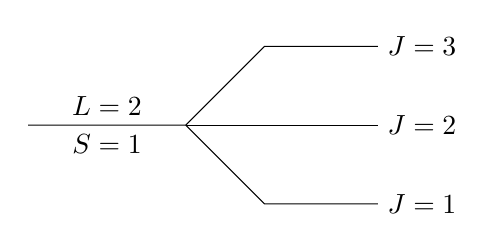
\begin{tikzpicture}
		% Termschema
		\node at (5,1) (J3) {$J=3$};
		\node at (5,0) (J2) {$J=2$};
		\node at (5,-1) (J1) {$J=1$};
		
		\draw (0,0) -- (2,0) node [midway, above] (TextNode) {$L=2$} node [midway, below] (TextNode) {$S=1$} -- (3,1) -- (J3);
		\draw (2,0) -- (J2);
		\draw (2,0) -- (3, -1) -- (J1);
	\end{tikzpicture}
	\caption{Termschema}
	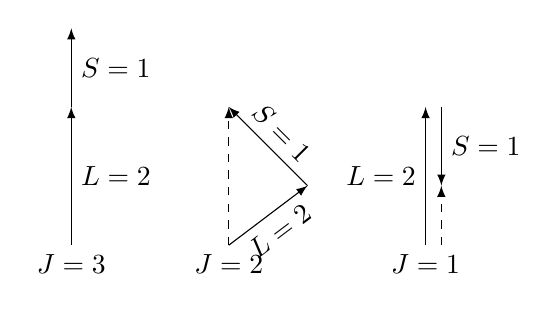
\begin{tikzpicture}
		%Vektordiagramme
		\node at (0,-2) (J3) {$J=3$};
		\draw [->, >=latex] (J3) -- (0,0) node [midway, right] (TextNode) {$L=2$};
		\draw [->, >=latex] (0,0) -- (0,1) node [midway, right] (TextNode) {$S=1$}; 
		
		\node at (2, -2) (J2) {$J=2$};
		\draw [->, >=latex] (J2.north) -- (3,-1) node [midway, below, sloped] {$L=2$};
		\draw [->, >=latex] (3,-1) -- (2,0) node [midway, above, sloped] {$S=1$};
		\draw [dashed, ->, >=latex] (J2) -- (2,0); 
		
		\node at (4.5, -2) (J1) {$J=1$};
		\draw [->, >=latex] (J1) -- (4.5,0) node [midway, left] {$L=2$};
		\draw [dashed, ->, >=latex] ([xshift=0.2 cm] J1.north) -- (4.7, -1);
		\draw [->, >=latex] (4.7, 0) -- (4.7, -1) node [midway, right] {$S=1$}; 
	\end{tikzpicture}
	\caption{Vektordiagramme der möglichen Additionen}
\end{figure}

Die Feinstruktur ist sehr klein verglichen mit den Energiedifferenzen zwischen verschiedenen $L_S$ oder $S$.\\

Im allgemeinen Fall gilt für die Energien: 
\begin{equation}
	E_j\lp n,L,S \rp = E\lp n,L,S \rp + c\cdot L\cdot S = E\lp n,L,S \rp + \frac{c}{2}\lp J(J+1) - S(S+1) - L(L+1) \rp
\end{equation}
	In diesem Beispiel folgt also mit L=1,S=1
\begin{equation}
	E_j(n,L,S) = E(n,L,S) + \frac{c}{2} \lp J(J+1) -8 \rp \hslash^2
\end{equation}
\begin{align*}
	\rightarrow J=3 &: E(n,L,S) + 2c\hslash^2\\
	J=2 &: E(n,L,S) - 1c\hslash^2\\
	J=1 &: E(n,L,S) - 3c\hslash^2
\end{align*}

c ist am größten für kleine n. $\rightarrow$ Bei großen n nur noch sehr kleine Feinstruktur.
\newpage
\subsection*{jj-Kopplung}

\subsubsection*{SATZ:}
Sei die Spin-Bahn-Kopplung eines Elektrons $\gg$ Bahn-Bahn-Kopplung und Spin-Spin-Kopplung verschiedener Elektronen. Dann ist der Gesamtdrehimpuls:
$$ \vec{J} = \sum_i \vec{j}_i = \sum_i \left(\vec{s}_i + \vec{\ell}_i \right)$$

\begin{itemize}
	\item Bei jj-Kopplung sind $L$ und $S$ nicht definiert, daher nur Gesamtdrehimpuls $J$
	\item Multiplett-Zustände nicht mehr erkennbar.
\end{itemize}

\begin{figure}[!h]
	\centering
	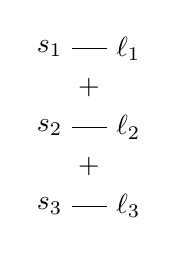
\begin{tikzpicture}
		\node at (0,0) (s1) {$s_1$};
		\node at (0,-1) (s2) {$s_2$};
		\node at (0,-2) (s3) {$s_3$};
		\node at (1,0) (l1) {$\ell_1$};
		\node at (1,-1) (l2) {$\ell_2$};
		\node at (1,-2) (l3) {$\ell_3$};
		\node at (0.5, -0.5) {$+$};
		\node at (0.5, -1.5) {$+$};
		
		\draw (s1) -- (l1);
		\draw (s2) -- (l2);
		\draw (s3) -- (l3);
	\end{tikzpicture}
	\caption{jj-Kopplung}
\end{figure}

\section{Clebsch-Gordan Koeffizienten \small{(ein kleiner Ausflug...)}}
\textbf{Von Michi} \newline 
Allgemeiner Basiswechsel in der Quantenmechanik:\\
Sei Vektor $\ket{\psi\ }$ in einer Basis $\mathcal{B}:= \left\{ \ket{b_1},\ ...,\ \ket{b_n}  \right\}$ gegeben durch:
\begin{equation}
	\ket{\psi\ } = \sum_{i=1}^{n} a_i \ket{b_i}
\end{equation}
$\Rightarrow$ Basisdarstellung in einer zweiten Basis $\mathcal{C}:= \left\{ \ket{c_1},\ ...,\ \ket{c_m} \right\}$ erhält man durch Multiplikation mit dem Eins--Operator in $\mathcal{C}$--Darstellung:
\begin{equation}
	\mathds{1}_{ \left\{ \mathcal{C} \right\} } = \sum_{j=1}^{m} \ket{c_i} \bra{c_i}
\end{equation}
\begin{align}
	\Rightarrow \ket{\psi} &= \mathds{1}_{ \left\{ \mathcal{C} \right\} } \ket{\psi} = \mathds{1}_{ \left\{ \mathcal{C} \right\} } \sum_{i=1}^{n} a_i \ket{b_i}\\
	\label{eq:1}
	&= \lp \sum_{j=1}^{m} \ket{c_j} \bra{c_j} \rp \sum_{i=1}^{n} a_i \ket{b_i} = \sum_{i,j} \underbrace{\vphantom{\sum} a_i \braket{c_j | b_i}}_{\mathclap{\text{Neue Koeffizienten von $\ket{\psi}$ in $\mathcal{C}$--Basis} }} \ket{c_j}
\end{align}
Die $\braket{c_j|b_i}$ nennt man auch ''Transformationsfunktionen''.\\

Wende dies nun auf die Addition von Drehimpulsen an:\\
Seien $\vec{X}_1,\ \vec{X}_2$ zwei verallgemeinerte Drehimpulse ($\vec{X}_i$ könnten z.B. Spins $ \vec{S}$, Bahndrehimpulse $\vec{L}$ oder totale Drehimpulse $\vec{J}$ sein). Dann existieren die zugehörigen Operatoren:
\begin{align*}
	&X_{1,z} \quad \vec{X}_1^2 \quad X_{2,z} \quad \vec{X}_2^2
	\intertext{mit den zugehörigen Quantenzahlen:}
	&m_1 \quad \kern 0.7em x_1 \quad \kern 0.4em m_2 \quad \kern 0.5em x_2
\end{align*}
wobei die $m_i$ die jeweiligen Projektionsquantenzahlen und die $x_i$ die Drehimpulsquantenzahlen sind.\\

Ein System, das durch diese beiden Drehimpulse beschrieben wird (z.B. ein $e^-$ mit Bahndrehimpuls und Spin) kann durch Vektoren der Form
\begin{equation}
	\ket{\psi} = \ket{x_1, m_1;\ x_2, m_2}
\end{equation}
vollständig beschrieben werden. Diese Vektoren sind Eigenzustände der Operatoren $X_{1,z},\ \vec{X}_1^2;\ X_{2,z},\ \vec{X}_2^2$.\\

Nun interessieren wir uns für den addierten Drehimpuls, der gegeben ist durch:
\begin{equation}
	\vec{X} = \vec{X}_1 + \vec{X}_2, \quad M_X = m_1 + m_2
\end{equation}
$\vec{X}$ besitzt analog zu $\vec{X}_1,\ \vec{X}_2$ entsprechende Operaton: $\vec{X}^2$ und $X_z$; jedoch sind die Vektoren $\ket{\psi} = \ket{x_1, m_1;\ x_2, m_2}$ keine Eigenzustände zu diesen beiden Operatoren. Um also eine einfache und übersichtliche Beschreibung des addierten Drehimpulses zu gewährleisten, suchen wir nun eine neue Basis, die aus Eigenvektoren von $\vec{X}^2,\ X_z$ besteht, also Vektoren der Form:
\begin{equation}
	\ket{\varphi} = \ket{X,\ M_X,\ x_1,\ x_2}
\end{equation}

Analog zu \ref{eq:1} ist die Basistransformation nun gegeben durch
\begin{equation}
	\ket{X, M_X, x_1, x_2} =\sum_{m_1,m_2} \ket{x_1, m_1, x_2, m_2} \cdot \braket{x_1, m_1, x_2,m_2|X, M_X, x_1, x_2}
\end{equation}
\textit{Hint: Vertauschen der beiden Produkte für besseres Verständnis und zur Anlogie zu Formel \ref{eq:1}}\\

Die Transformationsfunktion $\braket{x_1, m_1, x_2,m_2|X, M_X, x_1, x_2}$ gibt uns also die Koeffizienten (''CGK'') der Vektoren, welche die einzelnen Drehimpulse beschreiben, sodass deren Summe $\ket{X, M_X, x_1, x_2}$ ein Eigenzustand von $\vec{X}^2,\ X_z$ ist. 

\subsection*{Physikalische Interpretation der CGK}
\begin{equation}
	\left\vert \braket{x_1, m_1, x_2,m_2|X, M_X, x_1, x_2} \right\vert^2
\end{equation}
ist die Wahrscheinlichkeit, dass ein System der beiden Drehimpulse $\vec{X}_1,\ \vec{X}_2$ in der Konfiguration $m_1,\ m_2$ gefunden werden kann, wenn es den Gesamtdrehimpulsbetrag $X$ und Gesamt--z--Projektion $M_X$ hat. (Bedingte Wahrscheinlichkeit).\\

Die Berechnung der Clebsch-Gordan-Koeffizienten ist recht kompliziert\footnote{\href{https://de.wikipedia.org/wiki/Clebsch-Gordan-Koeffizient}{https://de.wikipedia.org/wiki/Clebsch-Gordan-Koeffizient}} \footnote{\href{https://en.wikipedia.org/wiki/Table_of_Clebsch?Gordan_coefficients}{https://en.wikipedia.org/wiki/Table\_of\_Clebsch?Gordan\_coefficients}}, weßhalb man sie auch in Tabellen nachschlagen kann (und sollte!).
\subsection*{Anleitung zum Lesen der Tabellen}
Meist ist eine Vielzahl kleinerer Tabellen angegeben. In der linken, oberen Ecke jeder dieser Tabellen steht ''$(x_1)\ x\ (x_2)$'', also die zwei Beträge der zu addierenden Drehimpulse.\\
Jede dieser Tabellen ist in mehrere Untertabellen gegliedert, diese haben die Form:
\begin{figure}[H]
	\centering
	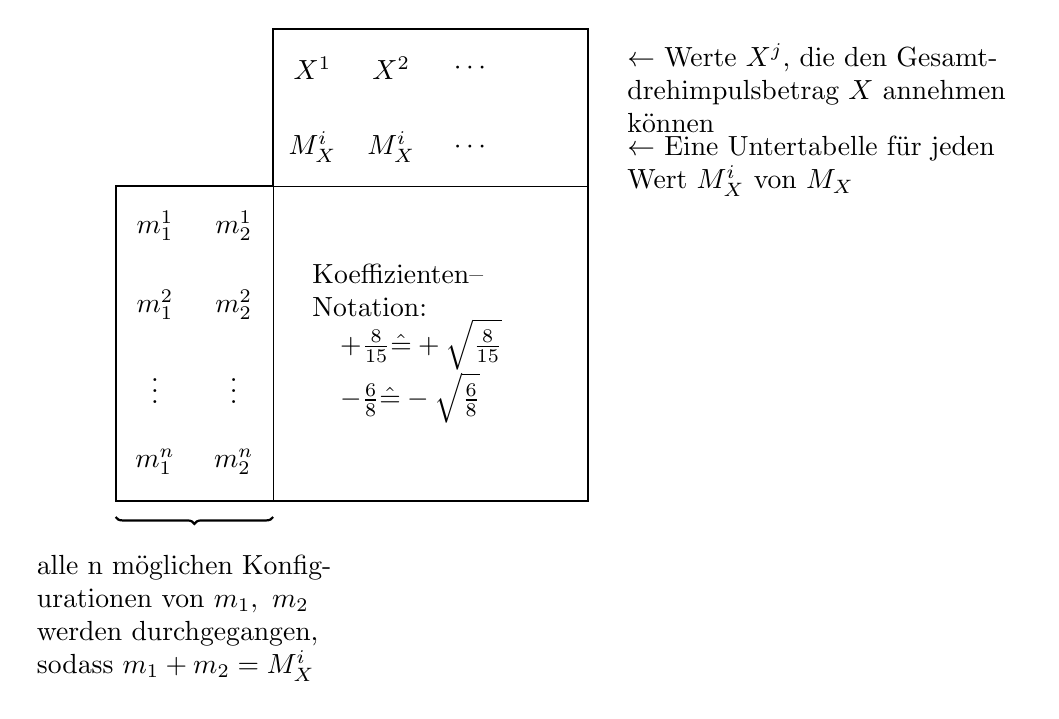
\begin{tikzpicture}
		%nodes
		\node at (0.5, 1.5) (x1) {$X^1$};
		\node at (1.5, 1.5) (x2) {$X^2$};
		\node at (0.5, 0.5) (Mxi1) {$M_X^i$};
		\node at (1.5, 0.5) (Mxi2) {$M_X^i$};
		\node at (2.5, 1.5) (dots1) {$\cdots$};
		\node at (2.5, 0.5) (dots2) {$\cdots$};
		\node at (-1.5, -0.5) (m11) {$m_1^1$};
		\node at (-0.5, -0.5) (m21) {$m_2^1$};
		\node at (-1.5, -1.5) (m12) {$m_1^2$};
		\node at (-0.5, -1.5) (m22) {$m_2^2$};
		\node at (-1.5, -2.5) (mdots1) {$\vdots$};
		\node at (-0.5, -2.5) (mdots2) {$\vdots$};
		\node at (-1.5, -3.5) (m1n) {$m_1^n$};
		\node at (-0.5, -3.5) (m2n) {$m_2^n$};
		%koeffizienten-node
		\node at (2, -2) [text width=3cm] (koeff) {Koeffizienten--Notation:\\ $\quad + \frac{8}{15} \hat{=} + \sqrt{\frac{8}{15}}$ \\ $\quad -\frac{6}{8} \hat{=} - \sqrt{\frac{6}{8}}$};
		%Bemerkungs-node
		\node at (7,1.25) (bem1) [text width=5cm] {$\leftarrow$ Werte $X^j$, die den Gesamtdrehimpulsbetrag $X$ annehmen können};
		\node at (7,0.25) (bem2) [text width=5cm] {$\leftarrow$ Eine Untertabelle für jeden Wert $M_X^i$ von $M_X$};
		%lines
		\draw [thick] (0,0) -- (0,2) -- (4,2) -- (4,-4) -- (-2,-4) -- (-2,0) -- cycle;
		\draw (4,0) -- (0,0) -- (0,-4);
		%underbrace
		\draw [thick, decoration={brace, mirror, raise=0.2cm}, decorate] (-2,-4) -- (0,-4) 
		node [pos=0.5,anchor=north,yshift=-0.55cm, text width=4cm] {alle n möglichen Konfigurationen von $m_1,\ m_2$ werden durchgegangen, sodass $m_1 + m_2 = M_X^i$}; 
	\end{tikzpicture}
	\caption{Schema einer CGK-Tabelle}
\end{figure}

\subsection*{Anmerkungen}
\begin{enumerate}
	\item Ein CG-Koeffizient, der physikalisch keinen Sinn ergibt (z.B. wenn $X \ge X_1 + X_2$ oder $M_X \neq m_1 + m_2$), ist null.\\
	Beispiel: $\braket{1,0,4,4|3,6,1,4}=0$\\
	weil: $0 (m_1) + 4(m_2) \neq 6 (M_X)$
	\item Am einfachsten kann man das Beschriebene anhand der Addition zweier Spins mit $s_1=s_2=\frac{1}{2}$ betrachten.\\
	So sieht man z.B. wie im Helium die Spin--Singulett und --Triplett Zustände zustande kommen. Man sieht auch, dass die CGK bestimmen, ob die Spinwellenfunktion symmetrisch oder antisymmetrisch ist.
\end{enumerate}
\end{document}